\section{Heuristics}
In the following both sections we present our heuristics that are based on the local-search optimization method \cite{aarts_2003,voss_2012}. The basic structure of such an algorithm is shown in \cref{alg:local_search}. Basically we first compute an initial solution from the input and afterwards improve it stepwise until some stopping criterion is met. In principle the stepwise improvements are performed locally to $sol$ such that each step yields a valid solution to our optimization problem. 
\begin{algorithm}[H]
\caption{A general framework of a local search heuristic.}
\label{alg:local_search}
\begin{algorithmic}[1]
  \Procedure{Local-Search}{$input$}
    \State $init$ := \Call{Compute-Initial-Solution}{$input$}
    \State $sol := init$
    \While{stopping criterion not met}
      \State x := \Call{Compute-Next-Neighbor-Solution}{$sol$}
      \If{$c(x) < c(sol)$}
        \State $sol := x$
      \EndIf
    \EndWhile
    \State \Return $sol$
  \EndProcedure
\end{algorithmic}
\end{algorithm}
One may interpret this by jumping from one point in the valid solution search space to another one in a certain local neighborhood. This interpretation is depicted in \cref{fig:local_search_illustration} where $s_0$ is the initial solution that we improve in a stepwise-manner by selecting a neighboring solution $s_1$ in its neighborhood $N(s_0)$. Obviously $s_1$ has lower total costs than $s_2$, however, depending on the neighborhood size $|N(s_0)|$ it may be a computationally demanding task. Therefore, while generating the neighboring solutions in $N(s_0)$ we terminate the search process as soon as we encounter a solution $s_1\in N(s_0)$ with $c(s_1) < c(s_0)$. This search strategy is called \emph{first-improvement} as we do not generate the best neighboring solution but are satisfied with any kind of improvement. This process is then continued until some stopping criterion is met. In particular, one may terminate after $i\in\mathbb{N}$ steps or in our case terminate as soon as $N(s_i)$ does not yield any improving solution, hence $s_i$ is called \emph{locally optimal}.
\begin{figure}[H]
  \centering
  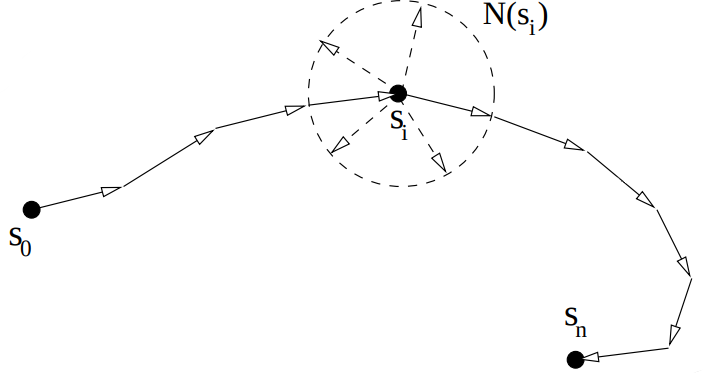
\includegraphics[width=0.7\linewidth]{./img/local_search.png}
  \caption{The search space where each point describes a valid solution to our optimization problem. We start from the initial solution $s_0$ improve it stepwise. For this matter we consider 'neighboring' solutions in $N(s_i)$ at the current solution $s_i$. When no neighboring solution is improving (i.e. has less total costs than current solution) we terminate our algorithm as $s_n$ is a locally optimal solution.}
  \label{fig:local_search_illustration}
\end{figure}

\ToDo{both cable in one, assign power automatically}

\subsection{Minimum Spanning Tree Approach}
The fact that each heliostat has to be connected to the solar tower $T$ with minimal costs infers utilizing a minimum spanning tree approach. We just need to consider the additional constraints of planarity as well as connectivity constraints. We thus choose Prim's algorithm \cite{prim_1957,cormen_2009} to compute an initial, valid solution to our problem. For the local search improvement steps we choose the \emph{cycle-neighborhood} function
\begin{equation*}
  N(T) := \{\tilde{T}\in\mathcal{T}|\}
\end{equation*}
